\documentclass{beamer}

\usepackage{tikz}
\usetikzlibrary{positioning,matrix, arrows.meta}
\usetikzlibrary{graphdrawing.trees}
\usetikzlibrary{external}
\tikzexternalize % activate!
\usepackage{color}
\newcommand{\vet}[1]{\foreach \num in {#1}{\el{\num}}}
\newcommand{\vetempty}[1]{\foreach \num in {#1}{\elempty{\num}}}
\newcommand{\el}[1]{\tikz{\node[font=\smaller, draw]{#1}}}
\newcommand{\elempty}[1]{\tikz{\node[font=\small, minimum size=1cm, draw=white, fill=white]{#1}}}
\newcommand{\bl}{\color{blue}}
\newcommand{\gr}{\color{gray}}
\newcommand{\re}{\color{red}}
\newcommand{\tcb}[1]{\textcolor{blue}{#1}}
\newcommand{\tcg}[1]{\textcolor{green}{#1}}
\newcommand{\tcr}[1]{\textcolor{red}{#1}}
\newcommand{\ar}{\tikz{\draw [->] (0,0) -- (0,0.4)}}
\newcommand{\nd}{\color{white!0}.}

\usepackage{beamerthemeSingapore}
\usepackage{graphicx}
%\usepackage{here}
\usepackage{url}
\usepackage[brazil]{babel}
\usepackage[T1]{fontenc}
\usepackage[utf8]{inputenc}
%\usepackage[tight,raggedright]{subfigure}
\usepackage{subfigure}
\usepackage[alf]{abntex2cite}
\usepackage{listings}
\usepackage{minted}
\usepackage{algorithm2e}
\usepackage{amsmath}
\usepackage{pdfpages}
% Please add the following required packages to your document preamble:
\usepackage{booktabs}
\usepackage{ragged2e}
\usepackage{etoolbox}
\usepackage{mathtools}
\usepackage{caption}
\usepackage{xmpmulti}

\tikzset{
  treenode/.style = {align=center, inner sep=0pt, text centered,
    font=\sffamily},
  arn_bf/.style = {treenode, rectangle, rounded corners=.8ex, black, font=\sffamily\bfseries, draw=black,fill=white, text width=3.5em, inner sep=2pt },% arbre rouge noir, noeud noir
  arn_rf/.style = {treenode, rectangle, rounded corners=.8ex, red, font=\sffamily\bfseries, draw=red,fill=white, text width=3.5em, inner sep=2pt },% arbre rouge noir, noeud noir
  arn_bt/.style = {treenode, rectangle, rounded corners=.8ex, black, font=\sffamily\bfseries, draw=black,fill=white, text width=2.5em, inner sep=2pt },% arbre rouge noir, noeud noir
  arn_rt/.style = {treenode, rectangle, rounded corners=.8ex, red, font=\sffamily\bfseries, draw=red,fill=white, text width=2.5em, inner sep=2pt },% arbre rouge noir, noeud noir
  arn_b/.style = {treenode, circle, black, font=\sffamily\bfseries, draw=black,
    fill=white, text width=1.5em},% arbre rouge noir, noeud noir
  arn_bl/.style = {treenode, circle, blue, font=\sffamily\bfseries, draw=black,
    fill=white, text width=1.5em},% arbre rouge noir, noeud noir
  arn_n/.style = {treenode, circle, white, font=\sffamily\bfseries, draw=black,
    fill=black, text width=1.5em},% arbre rouge noir, noeud noir
  arn_r/.style = {treenode, circle, red, draw=red, 
    text width=1.5em, very thick},% arbre rouge noir, noeud rouge
  arn_x/.style = {treenode, rectangle, draw=black,
    minimum width=0.5em, minimum height=0.5em}% arbre rouge noir, nil
}

\captionsetup[figure]{labelformat=empty,textfont=smaller}

\DeclarePairedDelimiter{\ceil}{\lceil}{\rceil}

\apptocmd{\frame}{}{\justifying}{} % Allow optional arguments after frame.

\AtBeginSection[]{
  \begin{frame}
  \vfill
  \centering
  \begin{beamercolorbox}[sep=8pt,center,shadow=true,rounded=true]{title}
    \usebeamerfont{title}\insertsectionhead\par%
  \end{beamercolorbox}
  \vfill
  \end{frame}
}

% TODO TODO TODO TODO TODO TODO TODO
\title{10 - Tabelas Hash}
\author{Prof. Alex Kutzke}
\date{Setembro de 2025}

\begin{document}

% ==========================================
\begin{frame}
  \begin{center}
    % TODO TODO TODO TODO TODO TODO
    \large{Setor de Educação Profissional e Tecnológica}\\
    Tecnologia em Análise e Desenvolvimento de Sistemas\\
    \vspace{1cm}			
    \small{DS141 - Estruturas de Dados II}
  \end{center}
  \titlepage
  \small{
  \center Tradução adaptada dos slides presentes em [1]. Imagens e exemplos também retirados do mesmo material.

  [1] \url{https://algs4.cs.princeton.edu/lectures/keynote/34HashTables.pdf}}
\end{frame}
% ==========================================

% ==========================================
\begin{frame}[c]{Roteiro}
  \tableofcontents

\end{frame}
% ==========================================

\section{Motivação}

\begin{frame}
  \frametitle{Resumo Implementações Tabela de Símbolos}

  \begin{figure}[h]
    \centering
    
\includegraphics[width=\textwidth]{img/symbol_table_review.png}
    \caption{Fonte: \cite{sedgewick2014algorithms}}
  \end{figure}

  \scriptsize{Dá pra fazer melhor?}
  \pause
  \scriptsize{\tcb{Sim!} Mas com um acesso diferente aos dados.}
\end{frame}

\begin{frame}
  \frametitle{Tabelas Hash: estratégia básica}

  Armazenar os itens em uma tabela indexada (o índice é uma função da chave armazenada).

  \tcb{Função Hash}: Método para computar o índice de um array a partir de uma chave.
  
  \begin{figure}[h]
    \centering
    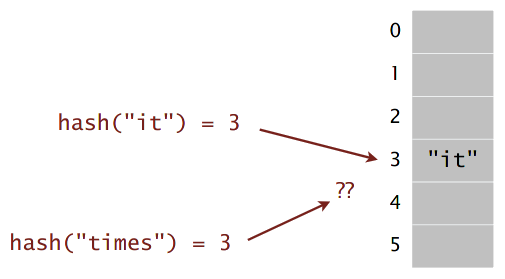
\includegraphics[width=.7\textwidth]{img/hash_function.png}
    \caption{Fonte: \cite{sedgewick2014algorithms}}
  \end{figure}

\end{frame}

\begin{frame}
  \frametitle{Tabelas Hash: estratégia básica}

  \tcb{Questões importantes:}
  \begin{itemize}
    \item Computar a função hash;
    \item Teste de igualdade: método para checar se duas chaves são iguais;
    \item Resolução de colisão: algoritmo e estruturas de dados para resolver o caso de quando duas ou mais chaves são alocadas em um mesmo índice do array.
  \end{itemize}
  
  \tcb{Relação clássica Armazenamento X Tempo}
  \begin{itemize}
    \item Sem limitação de espaço: função hash é trivial;
    \item Sem limitação de tempo: resolução de colisão é trivial (busca sequencial simples);
    \item Limitações de tempo e de espaço: hashing no mundo real. :)
  \end{itemize}
\end{frame}

\section{Funções Hash}

\begin{frame}
  \frametitle{Funções Hash}

  \tcb{Objetivo ideal}: Organizar as chaves uniformemente para produzir um índice.
  \begin{itemize}
    \item Eficientemente computável;
    \item Cada índice tem a mesma probabilidade de receber chaves.
  \end{itemize}

  \tcb{Exemplo}: Números de telefone (9 9999 9999).
  \begin{itemize}
    \item Ruim: primeiros três dígitos;
    \item Melhor: últimos três dígitos;
  \end{itemize}

  \tcb{Desafio prático}: Cada tipo de chave necessita de uma abordagem diferente.
\end{frame}

\begin{frame}
  \frametitle{Criando funções Hash}

  \begin{itemize}
    \item Algumas linguagens de programação já implementam funções hash para alguns tipos básicos:
    \begin{itemize}
      \item Java: \texttt{.hashcode()}
    \end{itemize}
    \item Diferentes estratégias podem ser utilizadas, dependendo do tipo de dado;
    \item Método mais comum: \tcb{hash modular}.
  \end{itemize}
\end{frame}

\begin{frame}
  \frametitle{Hash Modular}

  Dado um array (tabela) com $M$ posições, o \tcb{Hash Modular} se baseia no cálculo do módulo entre o valor da chave a ser armazenada e $M$:

  \[ hash(x) = x~mod~M \]

  Por exemplo, para $x = 98$ e $M = 10$:

  \[ hash(x) = 98~mod~10 = 8\]

  Assim, a chave 98 seria armazenada na posição 8 do array.

  \vspace{1cm}
  \tcb{Valor de M}: A escolha do tamanho do array tem um papel importante; Vejamos alguns exemplos.
\end{frame}

\begin{frame}
  \frametitle{Exemplo 1 Função Hash\\\small{Hash modular com chaves distribuídas uniformemente}}

  \begin{columns}
    \begin{column}{.5\textwidth}
      \[ h(x) = x~\%~12 \]

      \center Chaves a serem armazenadas:\\1, 2, 3, 4, 5, 6, 7, 8, 9, 10, 11, 12, 13, 14, 15, 16, 17, 18, 19, 20, 21, 22, 23.
    \end{column}
    \begin{column}{.5\textwidth}

      \begin{table}[]
        \centering
        \small
        \begin{tabular}{@{}cc@{}}
          \toprule
          Hashcode & Chave Armazenada \\ \midrule
          0        & 12, 24           \\
          1        & 1, 13            \\
          2        & 2, 14            \\
          3        & 3, 15            \\
          4        & 4, 16            \\
          5        & 5, 17            \\
          6        & 6, 18            \\
          7        & 7, 19            \\
          8        & 8, 20            \\
          9        & 9, 21            \\
          10       & 10, 22           \\
          11       & 11, 23           \\ \bottomrule
        \end{tabular}
      \end{table}  
    \end{column}
  \end{columns}
\end{frame}

\begin{frame}
  \frametitle{Exemplo 2 Função Hash\\\small{Hash modular com chaves NÃO distribuídas uniformemente}}

  \begin{columns}
    \begin{column}{.5\textwidth}
      \[ h(x) = x~\%~12 \]

      \center Chaves a serem armazenadas:\\3, 6, 9, 12, 15, 18, 21, 24, 27, 30, 33, 36, 39, 42, 45.
    \end{column}
    \begin{column}{.5\textwidth}

      \begin{table}[]
        \centering
        \small
        \begin{tabular}{@{}cc@{}}
          \toprule
          Hashcode & Chave Armazenada \\ \midrule
          0        & 12, 24, 36, 48   \\
          1        & --               \\
          2        & --               \\
          3        & 3, 15, 27, 39    \\
          4        & --               \\
          5        & --               \\
          6        & 6, 18, 30, 42    \\
          7        & --               \\
          8        & --               \\
          9        & 9, 21, 33, 45    \\
          10       & --               \\
          11       & --               \\ \bottomrule
        \end{tabular}
      \end{table}  
    \end{column}
  \end{columns}

  Como melhorar? \pause \tcb{Utilizar um valor primo para $M$}
\end{frame}

\begin{frame}
  \frametitle{Exemplo 3 Função Hash\\\small{Hash modular com chaves NÃO distribuídas uniformemente e M primo}}

  \begin{columns}
    \begin{column}{.5\textwidth}
      \[ h(x) = x~\%~11 \]

      \center Chaves a serem armazenadas:\\3, 6, 9, 12, 15, 18, 21, 24, 27, 30, 33, 36, 39, 42, 45.
    \end{column}
    \begin{column}{.5\textwidth}

      \begin{table}[]
        \centering
        \small
        \begin{tabular}{@{}cc@{}}
          \toprule
          Hashcode & Chave Armazenada \\ \midrule
          0        & 33               \\
          1        & 12, 45           \\
          2        & 24               \\
          3        & 3, 36            \\
          4        & 15               \\
          5        & 27               \\
          6        & 6, 39            \\
          7        & 18               \\
          8        & 30               \\
          9        & 9, 42            \\
          10       & 21               \\ \bottomrule
        \end{tabular}
      \end{table}  
    \end{column}
  \end{columns}
\end{frame}

\begin{frame}
  \frametitle{Exemplo 4 Função Hash\\\small{Hash modular para char's com chaves NÃO distribuídas uniformemente}}

  \begin{columns}
    \begin{column}{.5\textwidth}
      \[ h(x) = x~\%~9 \]

      \center Chaves a serem armazenadas:\\c, f, i, l, o, r, u, x.
      \begin{table}[]
        \centering
        \small
        \begin{tabular}{@{}cccc@{}}
          \toprule
          Char & Código ASCII & \% 9 & \% 7 \\ \midrule
          c    & 99           & 0    & 1    \\
          f    & 102          & 3    & 4    \\
          i    & 105          & 6    & 0    \\
          l    & 108          & 0    & 3    \\
          o    & 111          & 3    & 6    \\
          r    & 114          & 6    & 2    \\
          y    & 117          & 0    & 5    \\
          x    & 120          & 3    & 1    \\ \bottomrule
        \end{tabular}
      \end{table}  
    \end{column}
    \begin{column}{.5\textwidth}

      \begin{table}[]
        \centering
        \small
        \begin{tabular}{@{}cc@{}}
          \toprule
          Hashcode & Chave Armazenada \\ \midrule
          0        & c, l, u          \\
          1        & --               \\
          2        & --               \\
          3        & f, o, x          \\
          4        & --               \\
          5        & --               \\
          6        & i, r             \\
          7        & --               \\
          8        & --               \\ \bottomrule
        \end{tabular}
      \end{table}  
    \end{column}
  \end{columns}
\end{frame}

\begin{frame}
  \frametitle{Exemplo 5 Função Hash\\\small{Hash modular para char's com chaves NÃO distribuídas uniformemente e M primo}}

  \begin{columns}
    \begin{column}{.5\textwidth}
      \[ h(x) = x~\%~7 \]

      \center Chaves a serem armazenadas:\\c, f, i, l, o, r, u, x.
      \begin{table}[]
        \centering
        \small
        \begin{tabular}{@{}cccc@{}}
          \toprule
          Char & Código ASCII & \% 9 & \% 7 \\ \midrule
          c    & 99           & 0    & 1    \\
          f    & 102          & 3    & 4    \\
          i    & 105          & 6    & 0    \\
          l    & 108          & 0    & 3    \\
          o    & 111          & 3    & 6    \\
          r    & 114          & 6    & 2    \\
          y    & 117          & 0    & 5    \\
          x    & 120          & 3    & 1    \\ \bottomrule
        \end{tabular}
      \end{table}  
    \end{column}
    \begin{column}{.5\textwidth}

      \begin{table}[]
        \centering
        \small
        \begin{tabular}{@{}cc@{}}
          \toprule
          Hashcode & Chave Armazenada \\ \midrule
          0        & i                \\
          1        & c, x             \\
          2        & r                \\
          3        & l                \\
          4        & f                \\
          5        & u                \\
          6        & o                \\ \bottomrule
        \end{tabular}
      \end{table}  
    \end{column}
  \end{columns}
\end{frame}

\begin{frame}
  \frametitle{Chaves complexas}

  O hash modular pode ser utilizado para tipos simples de dados, mas também \textbf{para tipos complexos};
  \begin{itemize}
    \item Estratégia comum: separar a chave em partes, realizar o hash modular em cada parte e depois combinar os hashs obtidos em um único;
    \item Teoria semelhante à conversão de números para bases diferentes:
    \begin{itemize}
      \item Por exemplo, de binário para decimal;
      \item Cada dígito do número binário seria ``uma parte'' da chave:
    \end{itemize}
  \end{itemize}
  
  \[ 10101_{2} = 1 * 2^4 + 0 * 2^3 + 1 * 2^2 + 0 * 2^1 + 1 * 2^0 = 21_{10} \]

\end{frame}

\begin{frame}
  \frametitle{Exemplo: hash para strings}

  Para strings, podemos considerar cada carácter como ``uma parte'' do string. Considere uma string $s$ de tamanho $n$ e uma tabela de $m$ posições \cite{cpalg}:

  \begin{equation} \label{eq1}
    \begin{split}
      hash(s) & = s[0] + s[1]*p + s[2]*p^2 + \ldots + s[n−1]*p^{n-1}~mod~M \\
      & = \sum_{i=0}^{n-1}{s[i] * p^{i}}~mod~M
    \end{split}
	\end{equation}

  \begin{itemize}
    \item $p$ seria como o valor da base na conversão de números;
    \item Pode ser um número primo próximo ao número de letras do alfabeto considerado. Por exemplo, para o idioma inglês:
      \begin{itemize}
        \item $p = 31$ para apenas letras minúsculas;
        \item $p = 53$ para letras minúsculas e maiúsculas.
      \end{itemize}
  \end{itemize}

\end{frame}

\begin{frame}[fragile]
  \frametitle{Implementação: hash para strings}

  Uma possível implementação:
  \begin{minted}[frame=lines,framesep=2mm,baselinestretch=1,fontsize=\normalsize,linenos]{c}
int string_hash(char * s) {
  char c;
  int p = 31, m = 97;
  int hash_value = 0, p_pow = 1;

  while (c = *s++){
    hash_value = (hash_value + 
                  (c - 'a' + 1) * p_pow) % m;
    p_pow = p_pow * p;
  }
  return(hash_value);
}
  \end{minted}

\end{frame}

\begin{frame}
  \frametitle{Propriedades importantes de Funções Hash}

  \begin{itemize}
    \item Para duas chaves iguais, o valor da função hash deve ser o mesmo;
    \item O oposto não precisa ser verdadeiro:
    \begin{itemize}
      \item Se $t \neq s$, não há problemas se $hash(t) = hash(s)$;
      \item Embora tente-se evitar ao máximo esse comportamento (evitar colisões);
    \end{itemize}
  \item Precisa ser calculada de maneira eficiente ($O(1)$ se possível);
  \end{itemize}
\end{frame}

\begin{frame}
  \frametitle{Exemplo hash para strings - Implementação do Java}

  \begin{figure}[h]
    \centering
    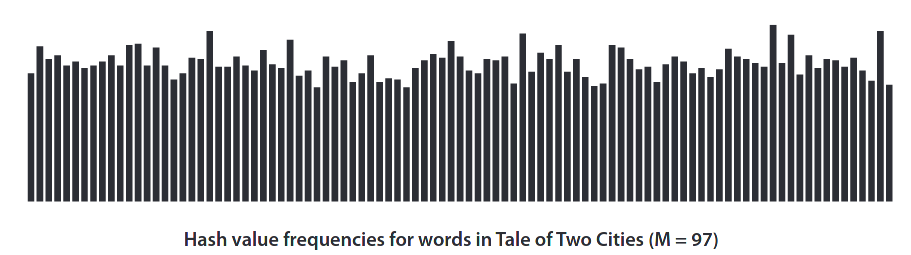
\includegraphics[width=\textwidth]{img/java_hash_string.png}
    \caption{Fonte: \cite{sedgewick2014algorithms}}
  \end{figure}

\end{frame}

\section{Encadeamento Externo (Separate Chaining)}

\begin{frame}
  \frametitle{Colisões}

  \tcb{Colisão}: Duas chaves diferentes recebem o mesmo valor hash.

  \begin{itemize}
    \item Ou temos memória suficiente para evitar esse tipo de problema;
    \item Ou utilizamos formas para tratar eficientemente eventuais colisões.
  \end{itemize}
  
  \begin{figure}[h]
    \centering
    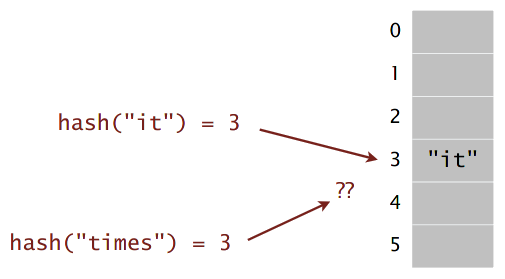
\includegraphics[width=.4\textwidth]{img/hash_function.png}
    \caption{Fonte: \cite{sedgewick2014algorithms}}
  \end{figure}

  Duas estratégias:
  \begin{itemize}
    \item Encadeamento externo (Separate Chaining);
    \item Encadeamento interno (Linear Probing).
  \end{itemize}

\end{frame}

\begin{frame}
  \frametitle{Encadeamento externo (Separate Chaining)}

  \tcb{Utilizar um array de $M < N$ listas ligadas}:
  \begin{itemize}
    \item Hash: mapeia uma chave para um inteiro $i$ entre $0$ e $M-1$;
    \item Inserção: inserir elemento na $i$-ésima lista (se já não estiver lá);
    \item Busca: pesquisa \textbf{apenas} na $i$-ésima lista.
  \end{itemize}
  
  \begin{figure}[h]
    \centering
    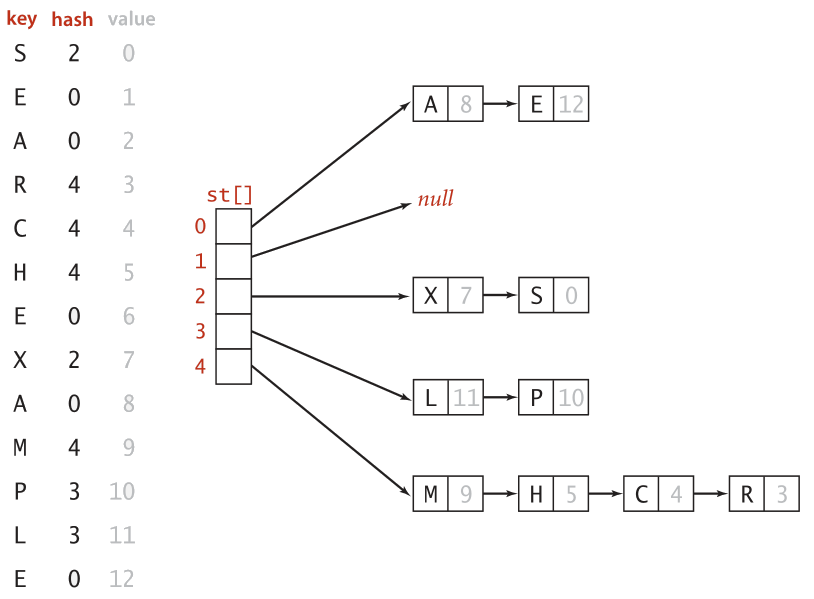
\includegraphics[width=.5\textwidth]{img/separate_chaining.png}
    \caption{Fonte: \cite{sedgewick2014algorithms}}
  \end{figure}

\end{frame}

\begin{frame}
  \frametitle{Análise}

  \tcb{Proposição}: Supondo uma função hash uniforme, a probabilidade de o número de itens em cada lista ser um fator constante de $N/M$ é muito próximo de $1$.
  
  \vspace{1cm}
  \tcb{Consequência}: Número de operações para busca/inserção é proporcional a $N/M$:
  \begin{itemize}
    \item $M$ muito grande $\rightarrow$ muitas listas vazias;
    \item $M$ muito pequeno $\rightarrow$ listas muito longas;
    \item Escolha típica $\rightarrow$ $M \sim N/4$ (\tcr{operações em tempo constante}).
  \end{itemize}

\end{frame}

\begin{frame}
  \frametitle{Redimensionamento da tabela}

  \tcb{Objetivo}: ter listas de tamanho médio $N/M$ (operações em tempo constante).
  \begin{itemize}
    \item Duplicar o tamanho da tabela M quando $N/M \ge 8$;
    \item Reduzir o tamanho da tabela M pela metade quando $N/M \le 8$;
    \item É necessário recalcular o hash de todos os elementos quando o tamanho da tabela é alterado. \textcolor{gray}{[\texttt{hash(x)} pode ser diferente para um M diferente]}
  \end{itemize}

\end{frame}

\begin{frame}
  \frametitle{Redimensionamento da tabela}

  \begin{figure}[h]
    \centering
    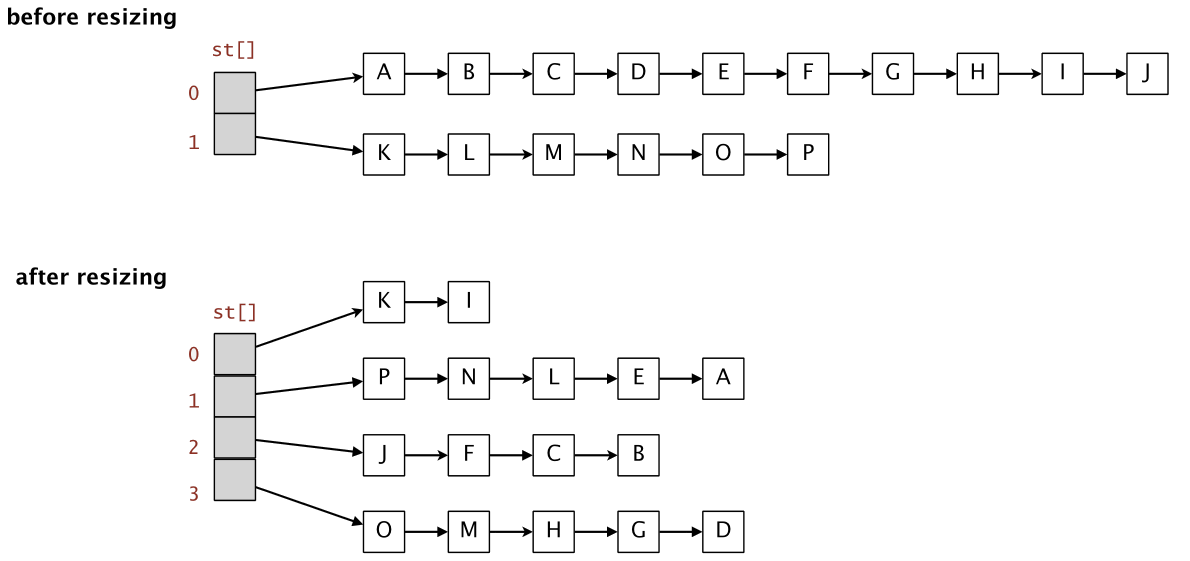
\includegraphics[width=\textwidth]{img/separate_chaining_resizing.png}
    \caption{Fonte: \cite{sedgewick2014algorithms}}
  \end{figure}

\end{frame}

\begin{frame}
  \frametitle{Remoção}

  \tcb{Q}: como remover uma chave da tabela?\\
  \tcb{R}: remoção simples da lista que contém o elemento.

  \begin{figure}[h]
    \centering
    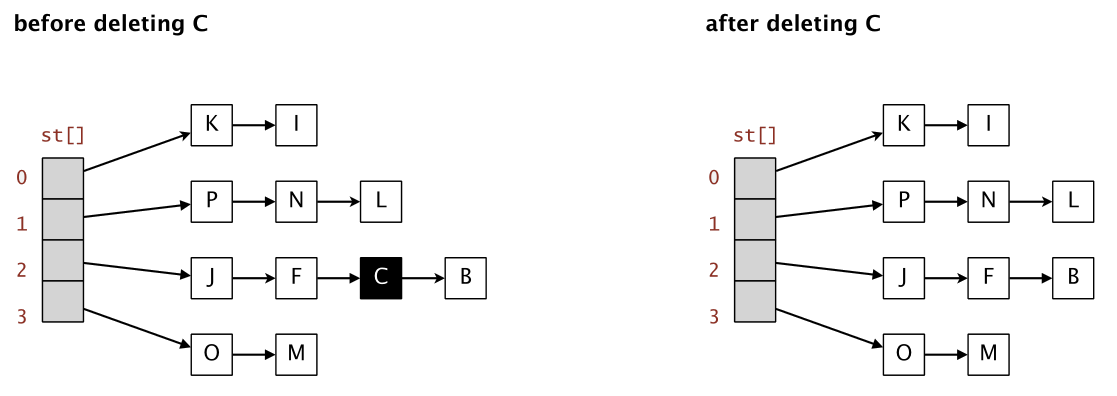
\includegraphics[width=\textwidth]{img/separate_chaining_deletion.png}
    \caption{Fonte: \cite{sedgewick2014algorithms}}
  \end{figure}

\end{frame}

\begin{frame}
  \frametitle{Resumo Implementações Tabela de Símbolos}

  \begin{figure}[h]
    \centering
    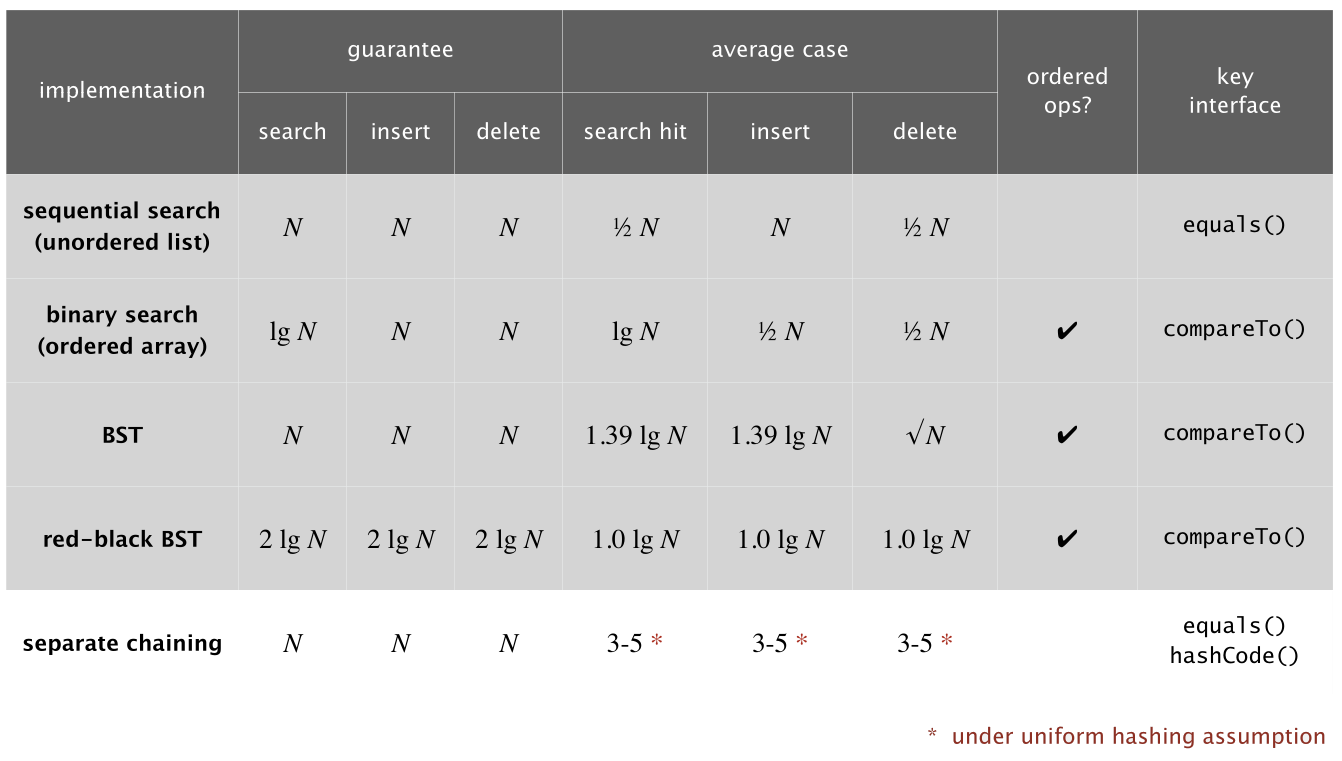
\includegraphics[width=\textwidth]{img/symbol_table_review2.png}
    \caption{Fonte: \cite{sedgewick2014algorithms}}
  \end{figure}
\end{frame}

\section{Encadeamento Interno (Linear Probing)}

\begin{frame}
  \frametitle{Encadeamento Interno (Linear Probing)}

  \tcb{Definição}: Quando uma nova chave colide, encontre o \textbf{próximo} espaço disponível na tabela.

  \begin{figure}[h]
    \centering
    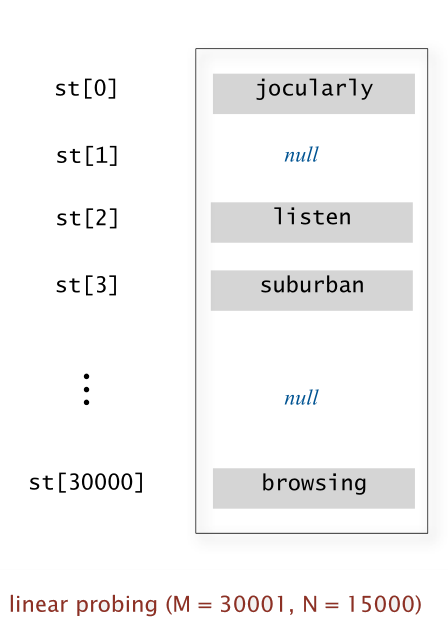
\includegraphics[width=.5\textheight]{img/linear_probing.png}
    \caption{Fonte: \cite{sedgewick2014algorithms}}
  \end{figure}
\end{frame}

\begin{frame}
  \frametitle{Encadeamento Interno (Linear Probing)}

  \begin{itemize}
    \item Hash: mapeia uma chave para um inteiro $i$ entre $0$ e $M-1$;
    \item Inserção: inserir elemento na $i$-ésima posição da tabela; se ocupado, procurar próxima posição livre;
    \item Busca: pesquisar na $i$-ésima posição da tabela; se ocupado mas não encontrado, buscar em $i+1$, $i+2$, etc.
  \end{itemize}

  \vspace{1cm}

  \pause
  \tcb{Nota}: Tamanho de $M$ \tcr{deve} ser maior do que o número de chaves $N$.
\end{frame}
  
\begin{frame}
  \frametitle{Exemplo}
  \begin{figure}[h]
    \centering
    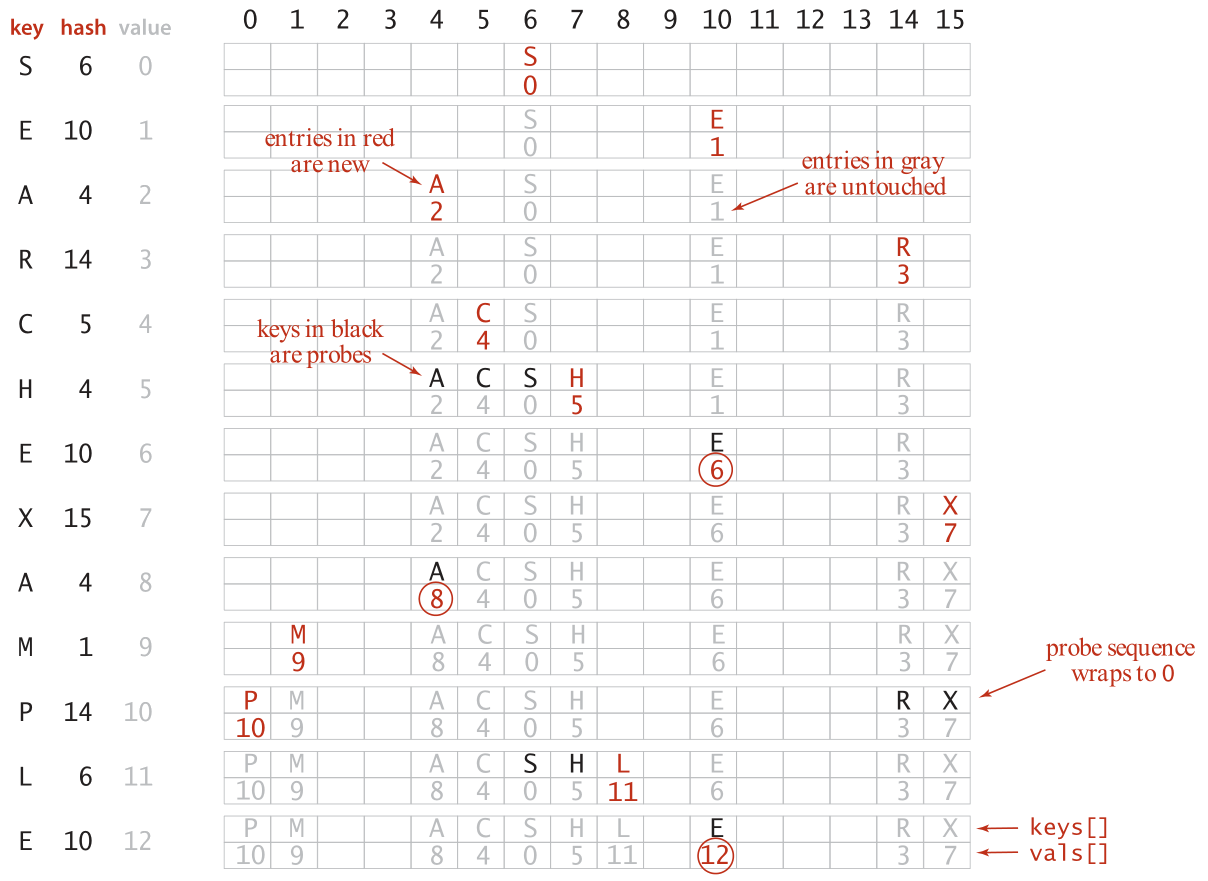
\includegraphics[width=.85\textwidth]{img/linear_probing_example.png}
    \caption{Fonte: \cite{sedgewick2014algorithms}}
  \end{figure}

\end{frame}

\begin{frame}
  \frametitle{Clustering}

  \tcb{Cluster}: Um bloco contíguo de itens;
  \tcb{Importante}: Novas chaves tem mais chances de ``caírem'' em clusters grandes:

  \begin{figure}[h]
    \centering
    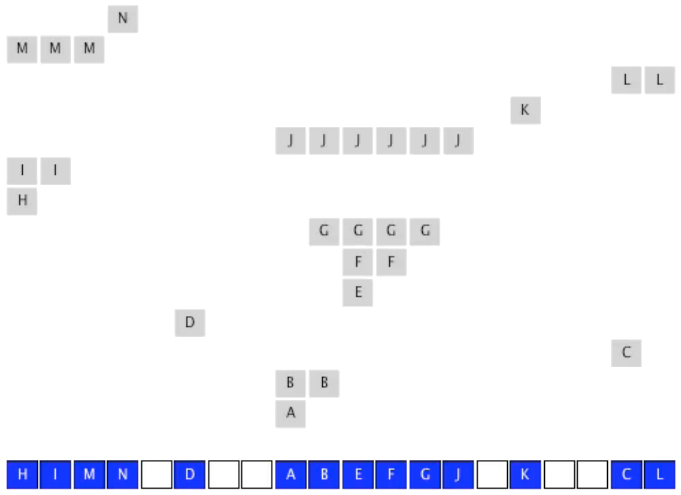
\includegraphics[width=.7\textheight]{img/linear_probing_clustering.png}
    \caption{Fonte: \cite{sedgewick2014algorithms}}
  \end{figure}
\end{frame}

\begin{frame}
  \frametitle{Clustering: exemplos}

  \begin{figure}[h]
    \centering
    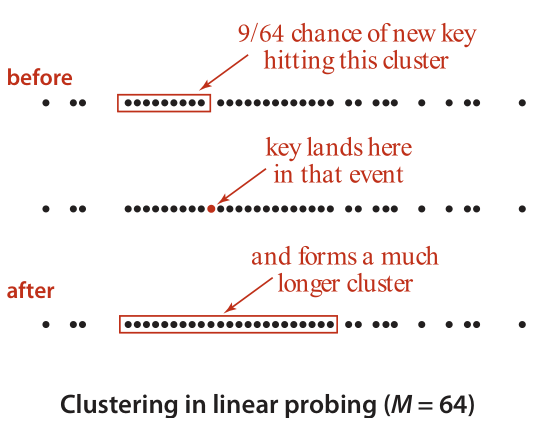
\includegraphics[width=.8\textheight]{img/linear_probing_clustering_ex_1.png}
    \caption{Fonte: \cite{sedgewick2014algorithms}}
  \end{figure}
\end{frame}

\begin{frame}
  \frametitle{Clustering: exemplos}

  \begin{figure}[h]
    \centering
    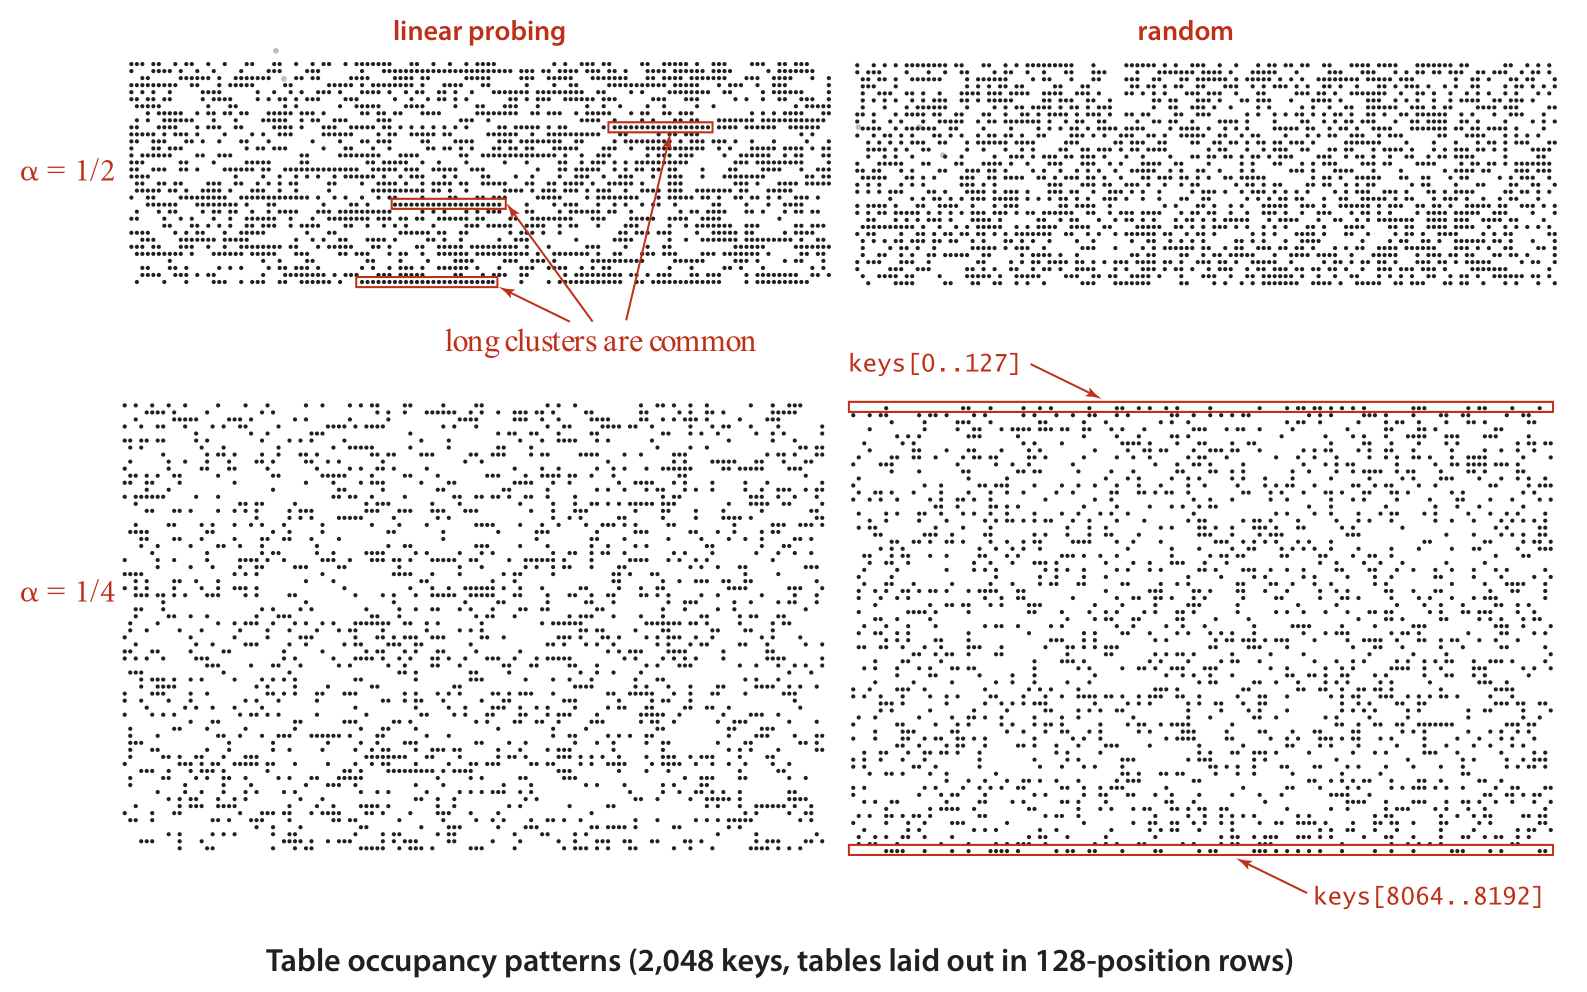
\includegraphics[width=.8\textwidth]{img/linear_probing_clustering_ex_2.png}
    \caption{Fonte: \cite{sedgewick2014algorithms}}
  \end{figure}
  $\alpha = N/M$
\end{frame}

\begin{frame}
  \frametitle{Análise}

  \tcb{Proposição}: Supondo uma função hash uniforme, o número médio de operações com encadeamento interno para uma tabela de tamanho $M$ que contém $N = \alpha M$ chaves é:\\

  Search hit:
  
  \[ \sim \frac{1}{2}(1+\frac{1}{1-\alpha}) \]

  Search miss/inserção:
  
  \[ \sim \frac{1}{2}(1+\frac{1}{(1-\alpha)^2}) \]

  \smaller{
  \tcb{Consequência}: Ou seja, constante, mas depende da manutenção da relação $\alpha = N/M$:
  \begin{itemize}
    \item $M$ muito grande $\rightarrow$ muitas posições vazias;
    \item $M$ muito pequeno $\rightarrow$ tempo de busca linear;
    \item Escolha típica $\rightarrow$ $\alpha = N/M \sim \frac{1}{2}$ (\tcr{operações para busca/inserção $\sim 5/2$}).
  \end{itemize}}

\end{frame}

\begin{frame}
  \frametitle{Redimensionamento da tabela}

  \tcb{Objetivo}: ter listas de tamanho médio $N/M \le \frac{1}{2}$
  \begin{itemize}
    \item Duplicar o tamanho da tabela M quando $N/M \ge \frac{1}{2}$;
    \item Reduzir o tamanho da tabela M pela metade quando $N/M \le \frac{1}{8}$;
    \item É necessário recalcular o hash de todos os elementos quando o tamanho da tabela é alterado. \textcolor{gray}{[\texttt{hash(x)} pode ser diferente para um M diferente]}
  \end{itemize}

\end{frame}

\begin{frame}
  \frametitle{Redimensionamento da tabela}

  \begin{figure}[h]
    \centering
    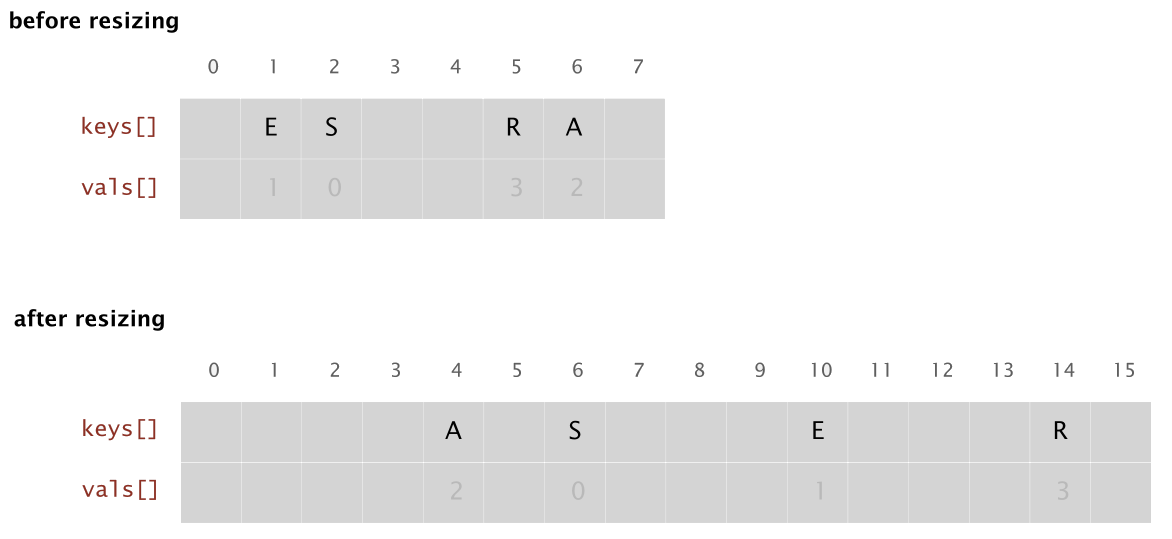
\includegraphics[width=\textwidth]{img/linear_probing_resizing.png}
    \caption{Fonte: \cite{sedgewick2014algorithms}}
  \end{figure}

\end{frame}

\begin{frame}
  \frametitle{Remoção}

  \tcb{Q}: como remover uma chave da tabela?\\
  \tcb{R}: exige um pouco de cuidado.

  \begin{figure}[h]
    \centering
    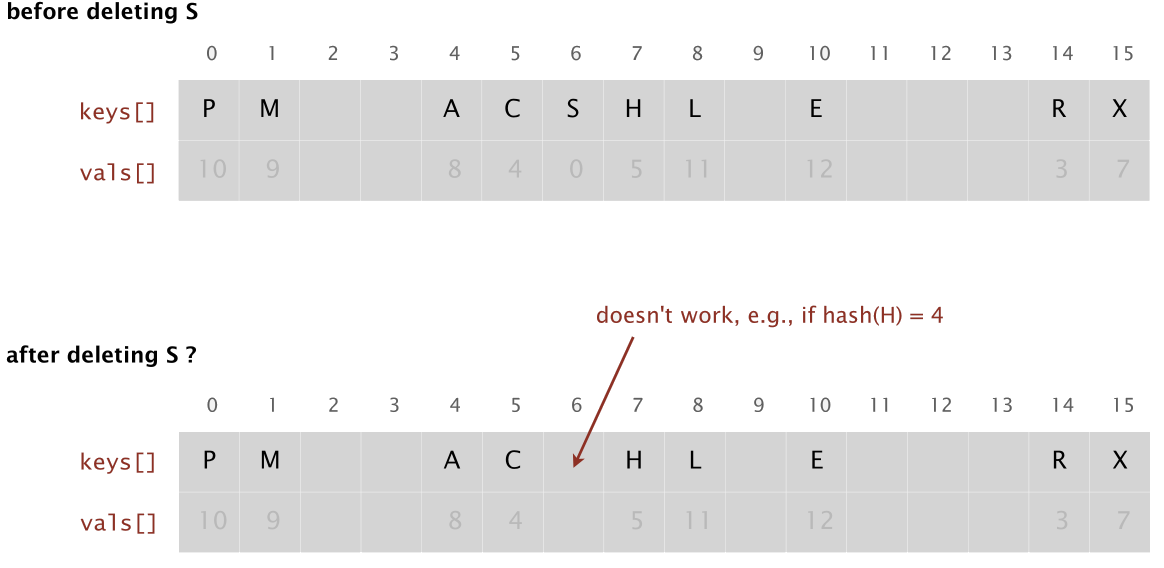
\includegraphics[width=\textwidth]{img/linear_probing_deletion.png}
    \caption{Fonte: \cite{sedgewick2014algorithms}}
  \end{figure}

\end{frame}

\begin{frame}
  \frametitle{Resumo Implementações Tabela de Símbolos}

  \begin{figure}[h]
    \centering
    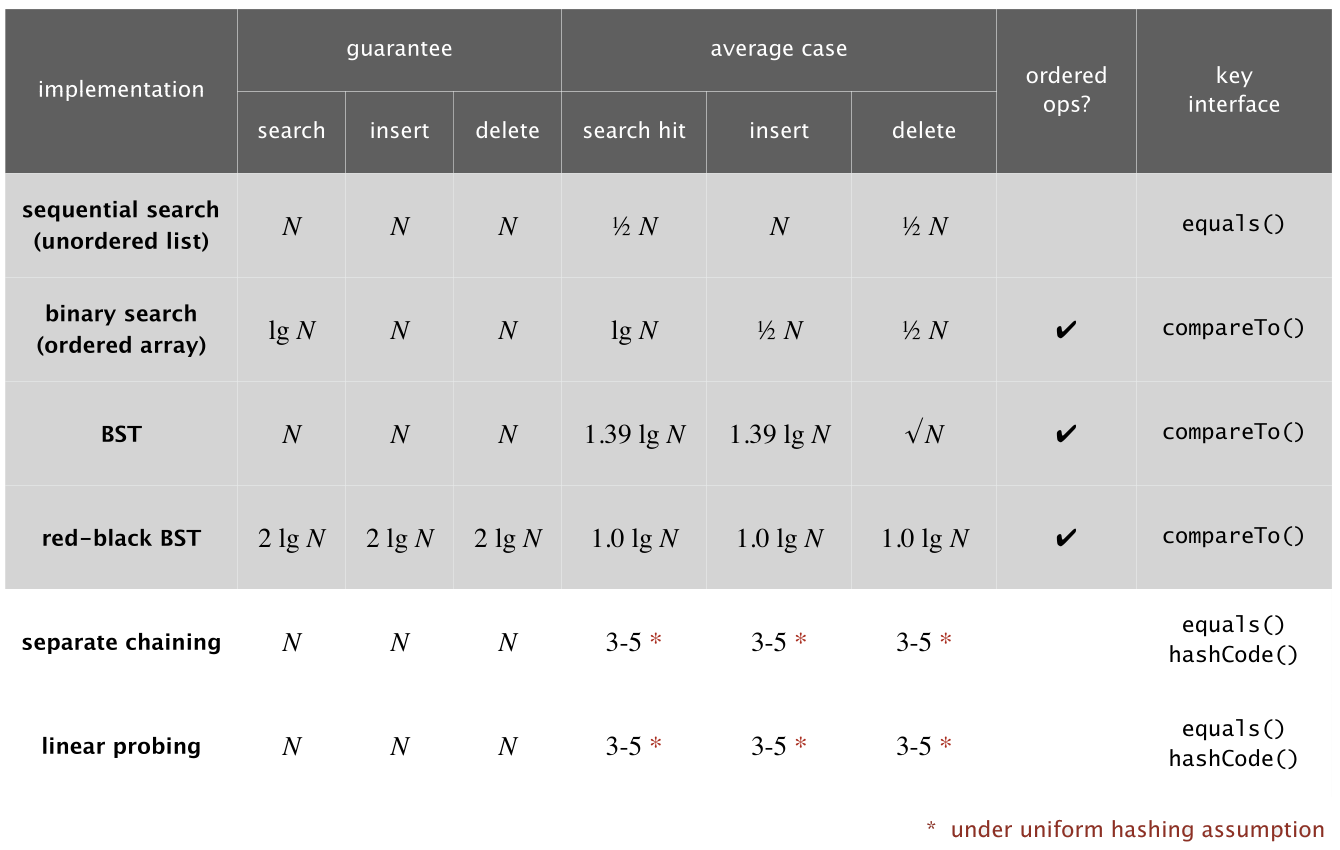
\includegraphics[width=\textwidth]{img/symbol_table_review3.png}
    \caption{Fonte: \cite{sedgewick2014algorithms}}
  \end{figure}
\end{frame}


\begin{frame}
  \frametitle{Referências utilizadas na apresentação}
  \bibliography{referencias}
\end{frame}
% ==========================================

\end{document}
